\chapter{State of the art}
This section presents the state of the art in navigation techniques for liver
surgery with a focus on approaches tackling the problems of registration during
liver surgeries and the challanges when creating 3D models of the liver
intraoperatively. Advantages and disadvatages of the different approaches are
presented and discussed.
\section{Ultrasound based registration of the liver}
\label{sec:ultrasoundBasedRegistration}

% \subsection{Rigid - Using the surface}
% laser range scan combine image and surface image-guided liver surgery \cite{cash2007concepts}

\subsection{Vessel based}
The liver vessels build a complex structure and are
therefore well suited for registration. Rigid as well as nonrigid registrations
have been studied based on liver vessels \cite{ribes2012image}\cite{lange20093d}. 
On intraoperative ultrasound images the
blood vessel sections are visible as black areas within the liver tissue and can
be segmented in real time by the use of fast algorithms \cite{ribes2012image}. Then the
vessels are 
reconstructed to a 3D US model and an iterative closest point (ICP) algorithm is used to align the vessel model to
the preoperative CT data. This method works on a small subvolume of the liver
and performs a local rigid registration. It helped to improve the
initial manual alignment in 8/14 datasets and in 2/14 the algorithm did not
converge \cite{ribes2012image}.
% The median alignment precision with
% this method was 6.3 mm averaged over 50 surgeries.

% \begin{figure}[H]
%   \centering
%  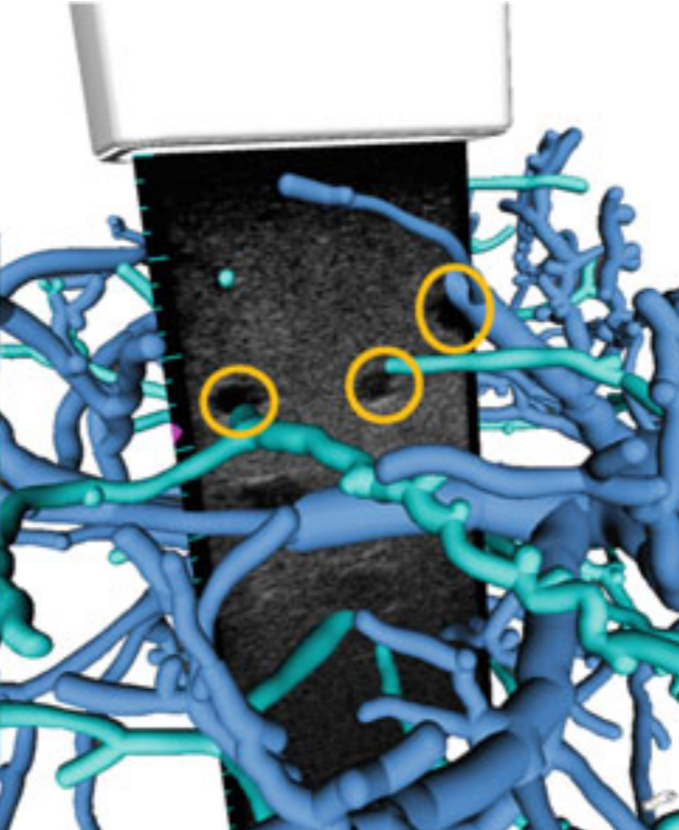
\includegraphics[width=0.3\textwidth]{VesselRegistration1}
%  \caption{Vessel based registration \cite{ribes2012image}}
%   \label{fig:VesselRegistration1}
% \end{figure}

% \begin{figure}[H]
%   \centering
%  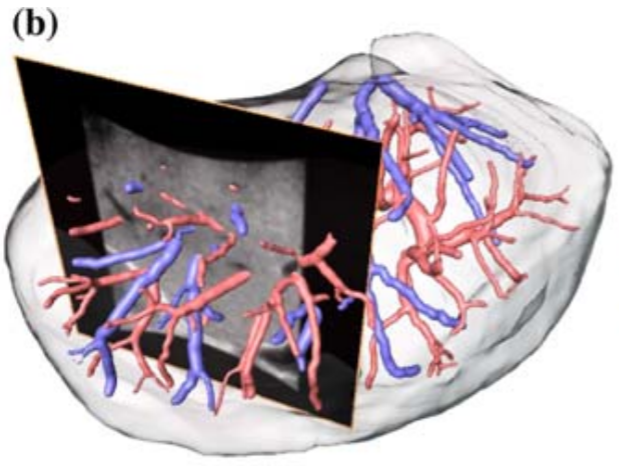
\includegraphics[width=0.4\textwidth]{VesselRegistration2}
%  \caption{Vessel based registration \cite{lange20093d}}
%   \label{fig:VesselRegistration2}
% \end{figure}

\begin{figure}[H]
  \centering
  \minipage{0.3\linewidth}
 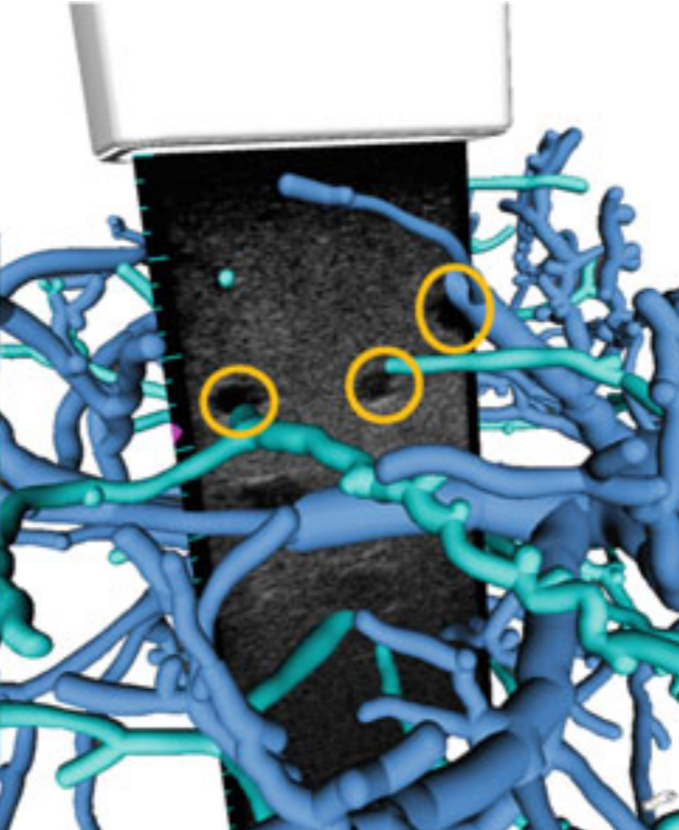
\includegraphics[width=\linewidth]{VesselRegistration1}
  \endminipage
  \hfill
  \minipage{0.48\linewidth}
 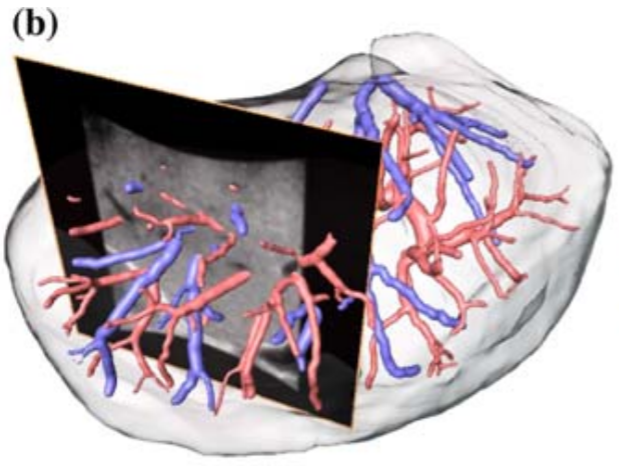
\includegraphics[width=\linewidth]{VesselRegistration2}
  \endminipage
  \hfill
 \caption{Vessel based registration: left \cite{ribes2012image}, right \cite{lange20093d}}
  \label{fig:VesselRegistration}
\end{figure}

% 3D ultrasound-CT registration of the liver (non-rigid) \cite{lange20093d}
% Surface based US/MeVis-CT registration for open liver surgery \cite{ribes1surface}
% Automatic registration of 3D ultrasound with pre-operative MeVis-CT (rigid)\cite{ribes2012image}

\subsection{Using the surface and vessels combined}
To combine the inner structure of the vessels with the surface of the liver is
an approach to create an automatic registration without the need of an initial
alignment. Nam et al. \cite{nam2011automatic} first segment the vessel lumens and the liver surface from 3D
B-mode ultrasound images. Then they use an edge matching algorithm to achieve an
automatic initial registration based on the vessels. The registration is
iteratively refined by jointly using the liver surface and vessel data (Figure
\ref{fig:SurfaceAndVesselRegistration}). The achieved average distance between
6-8 anatomical landmarks after automatic registration with this approach was 3.0 mm.

% Automatic registration between 3D intra-operative ultrasound and pre-operative
% CT images \cite{nam2011automatic}
\begin{figure}[H]
  \centering
 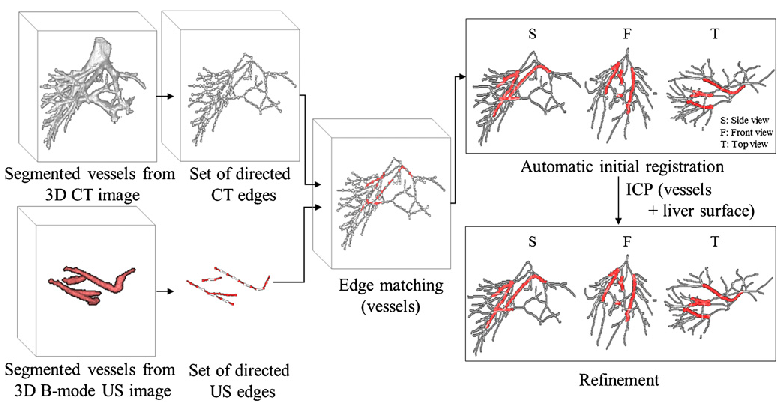
\includegraphics[width=0.8\textwidth]{SurfaceAndVesselRegistration}
 \caption{Surface and vessel based registration \cite{nam2011automatic}}
  \label{fig:SurfaceAndVesselRegistration}
\end{figure}


% Registration of organ surface (prostate surface) with intra-operative 3D ultrasound image using
%  genetic algorithm \cite{wu2003registration}


% \subsection{Nonrigid - Using the surface and a tumor}
% Nonrigid Registration Method
% for Liver Surgery Using Sparse Intraoperative Data (target registration error (TRE) of 3.3 mm for targets dispersed
% throughout the phantom volume) \cite{rucker2014mechanics}
% \begin{figure}[H]
%   \centering
%  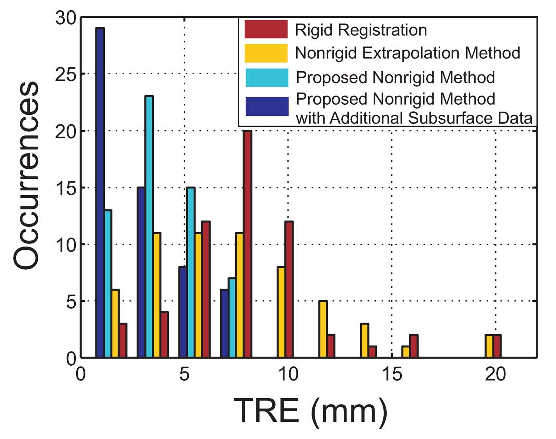
\includegraphics[width=0.6\textwidth]{SurfaceWithSubsurface}
%  \caption{Statistical histogramm of 58 target errors from different registration
%  methods applied to their representive phantom. Red: Rigid registration with an
%  ICP algorithm. Yellow: Rigid registration and afterwards nonrigid registration
%  using a surface Laplacian. Light blue: Rigid registration and afterwards
%  nonrigid registration using their new iterative method. Dark blue: Same as
%  light blue but with one additional subsurface point for the nonrigid
%  registration part. \cite{rucker2014mechanics}}
%   \label{fig:SurfaceWithSubsurface}
% \end{figure}

\section{Surface registration}
Surface registration is registration based on surfaces. It is used and studied
for several years in all kinds of fields \cite{ramos2015review}. Especially in
the field of medical technology, a lot of research is being done in the
direction of contactless registration. Intraoperatively, different camera technologies which lead
to depth images are used to sample the surface of an organ. Often used imaging systems are stereo cameras
\cite{furukawa2010accurate}, structured light \cite{salvi2004pattern} and
laser range scanners \cite{cash2003incorporation}. From these intraoperatively
created data sets, surfaces are reconstructed and then used for registration. To
find the mapping between the surfaces, mostly different variants of the iterative
closest point \cite{besl1992method} algorithm are used. 

These surface based methods are limited for different reasons. In most cases
only part of the whole organ can be seen (scanned). The scanned surface may lack
of unique structures on the surface. The scanning process can 
lead to noisy data. The organ of interest may be deformed between the
acquisitions of the surface samples. Therefore researchers try to compensate for
intraoperative soft-tissue deformations \cite{cash2005compensating}\cite{dagon2008real}.

\section{Creating models from intraoperative imaging for liver resection
  surgeries}
In the following subsections intraoperatively created models of parts of the
liver are presented. All presented approaches used their reconstructed parts to
register the surgical site to the preoperative data.
% \subsection{Prostate surface - Based on ultrasound}
% prostate surface \cite{wu2003registration}
% \begin{figure}[H]
%   \centering
%  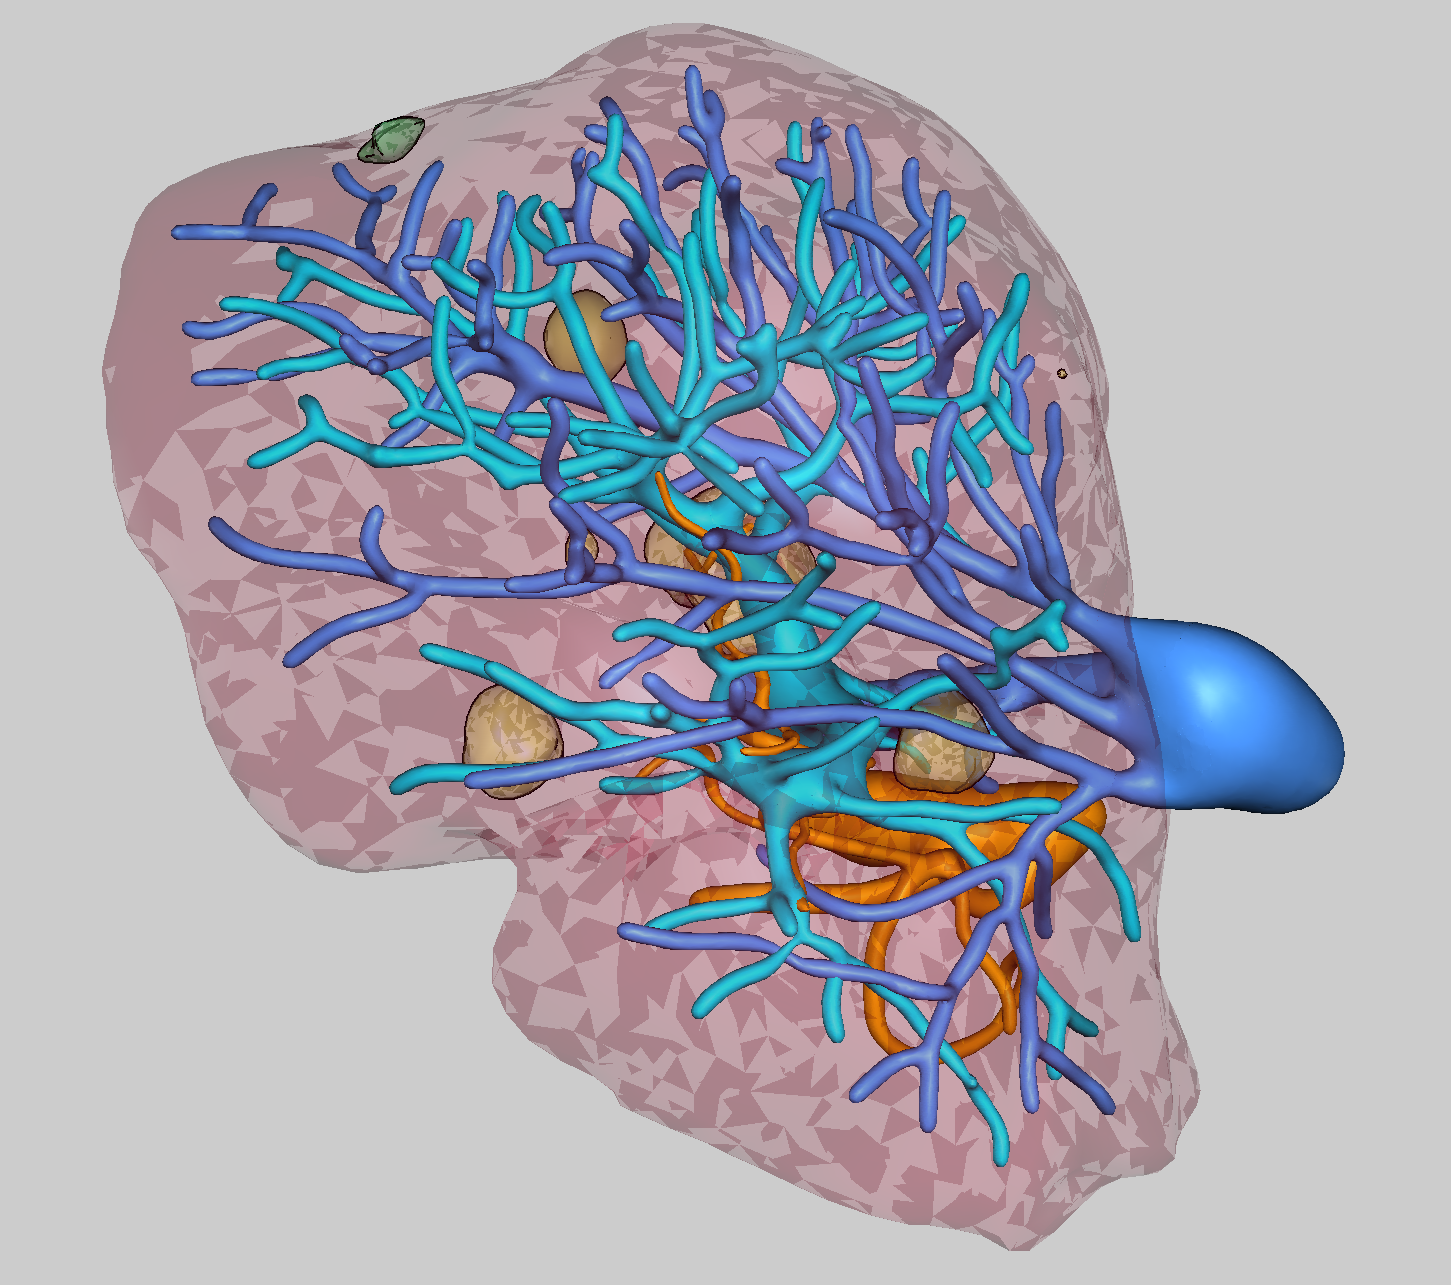
\includegraphics[width=0.6\textwidth]{MeVisExample}
%  \caption{Example of a preoperative 3D model created by MeVis}%DK patient
%   \label{fig:MeVisExample}
% \end{figure}


\subsection{Liver surface - Based on laser range scanner}
Laser range scanners achieve measurments with submillimetric errors and can rapidly
acquire thousands of 3D points. In addition to collecting dense surface points,
the scanner simultaneously takes images of the visible scene and texture maps
the color information onto each surface point (Figure \ref{fig:LaserRangeSurface}). 

The downside of such an approach is that the laser range scanner takes a lot of
space in the operating room and that it only captures the surface data visible
from one angle. In addition, only the surface can be reconstructed and no
internal structures of the liver.
% laser range scan combine image and surface image-guided liver surgery \cite{cash2007concepts}
\begin{figure}[H]
  \centering
 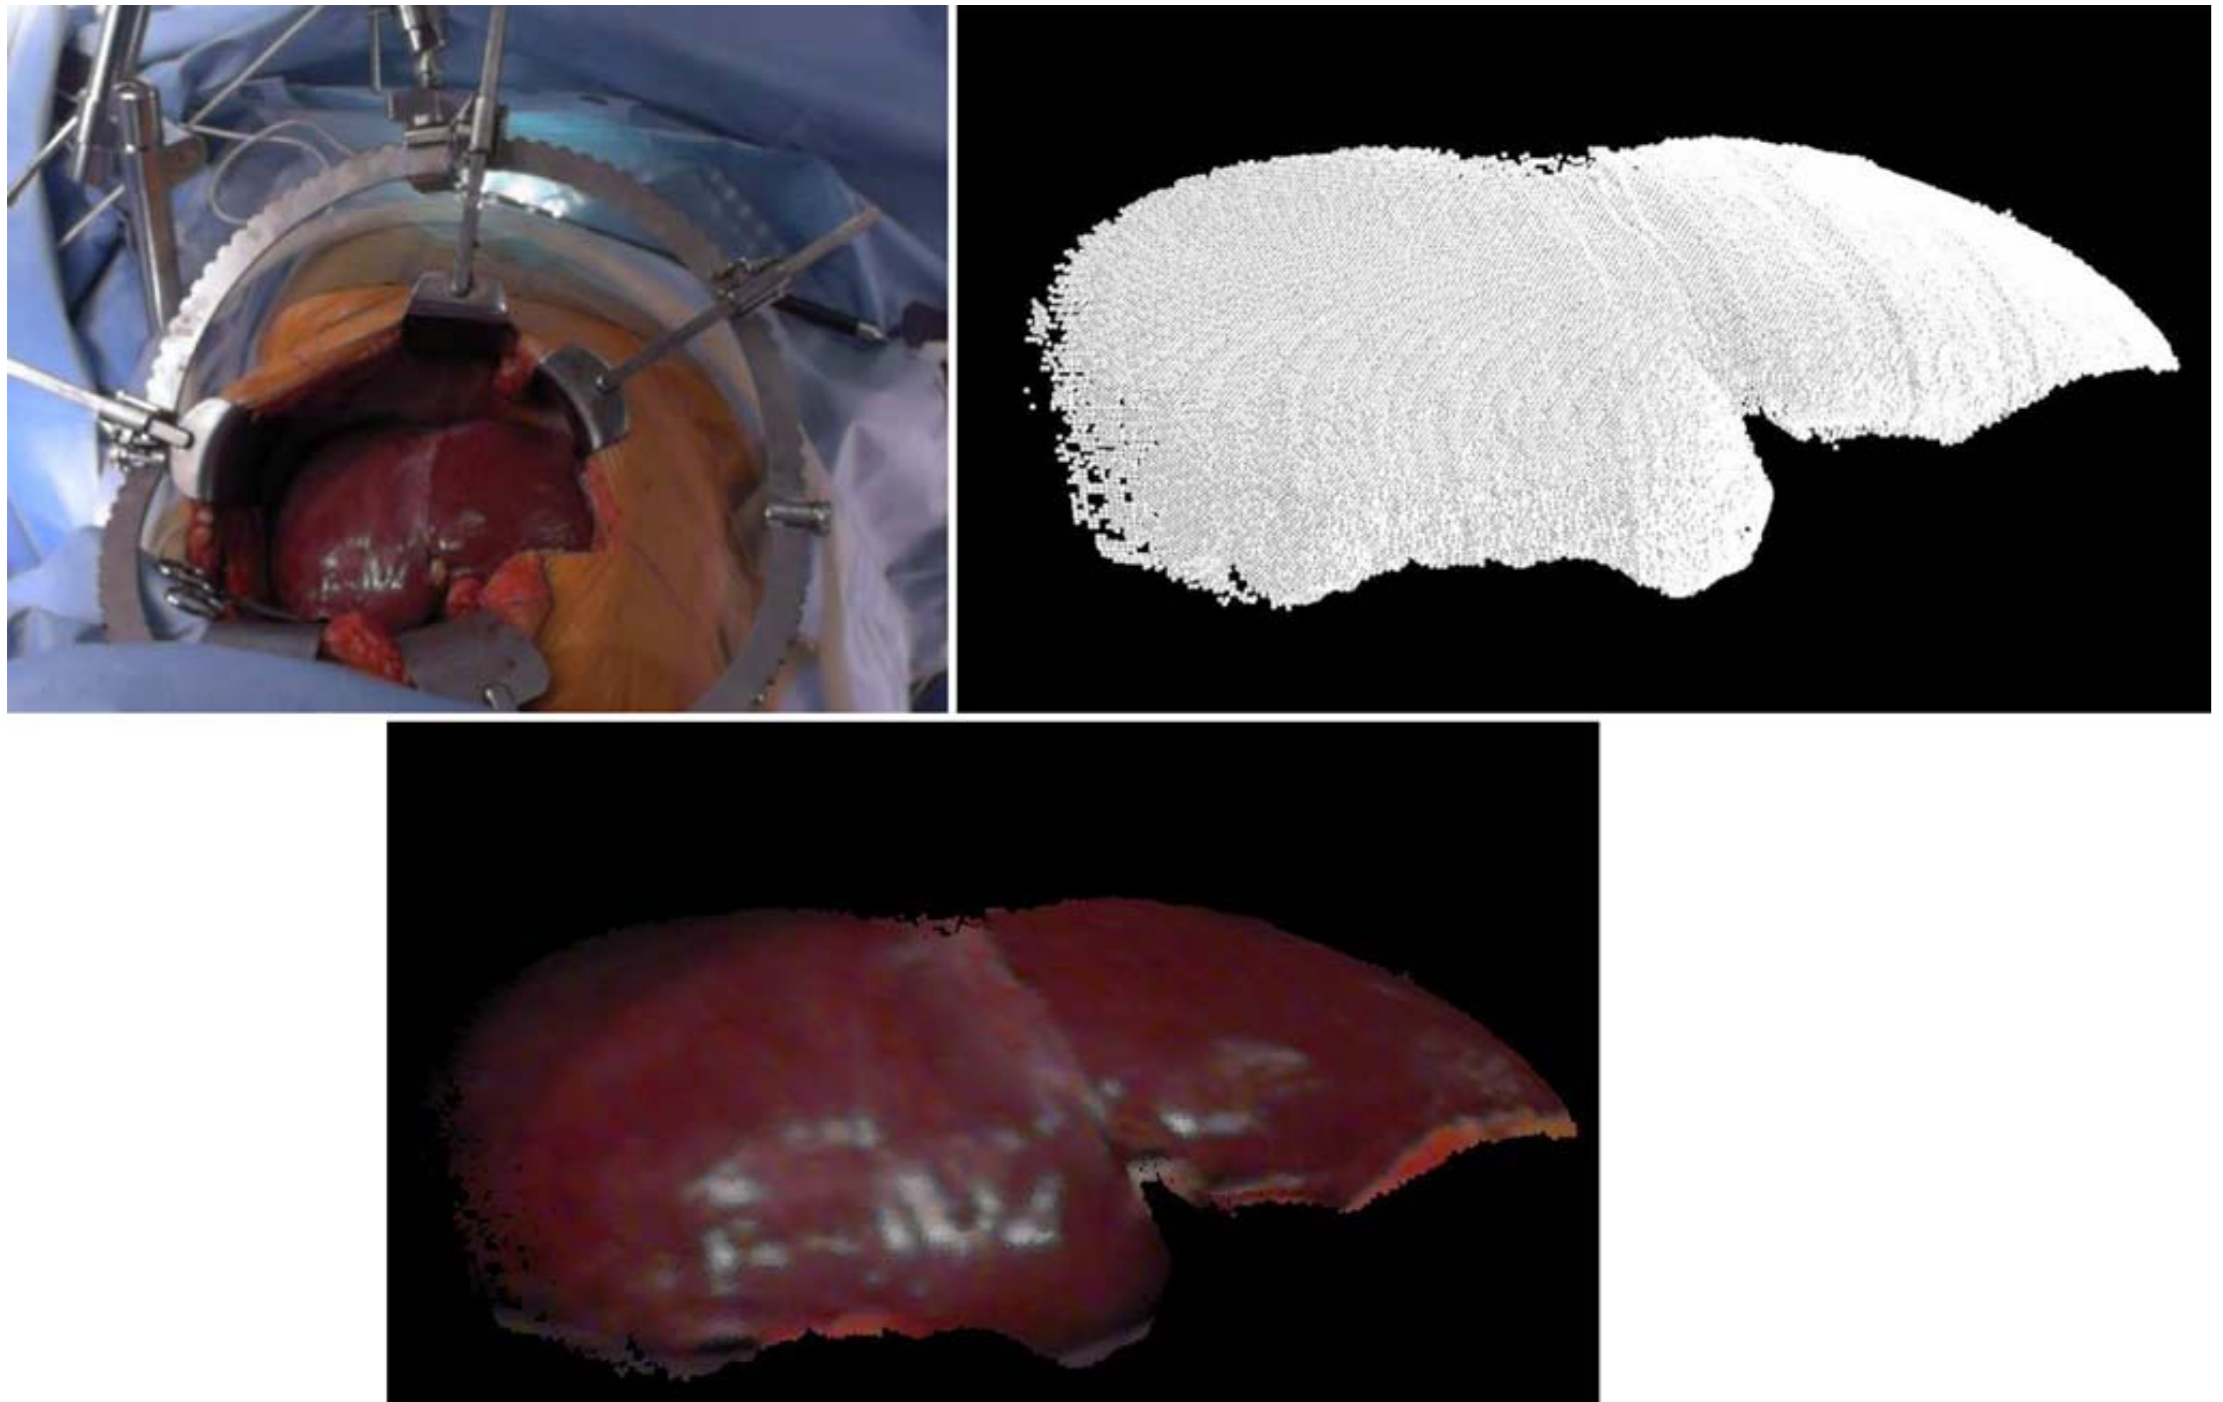
\includegraphics[width=0.8\textwidth]{LaserRangeSurface}
 \caption{Laser range scanning during open surgeries \cite{cash2007concepts}.
   Top left: This image shows that it is difficult to see a large part of the liver
   surface from one angle. Top right: The reconstructed surface. Bottom:
   Reconstructed surface combined with the texture map. }
  \label{fig:LaserRangeSurface}
\end{figure}

\subsection{Liver surface - Based on stereo endoscopic images}
This approach works for open surgeries as well as for laproscopic ones. They use
a optically tracked stereo endoscope to record the surface of the liver with 20
frames per second (FPS) intraoperatively and use
the images of each frame to create a dense depth image with subpixel precision \cite{speidel2011intraoperative}.
From these images the 3D surface positions are calculated. From the growing and resulting
point cloud the surface is reconstructed in real time (Figure \ref{fig:SurfaceReconstructionStereoBased}).

The disadvatage of this approach is that no internal structures are included in
the reconstruction of the intraoperative situation.
% Intraoperative surface reconstruction and
% biomechanical modeling for soft tissue registration \cite{speidel2011intraoperative}
\begin{figure}[H]
  \centering
 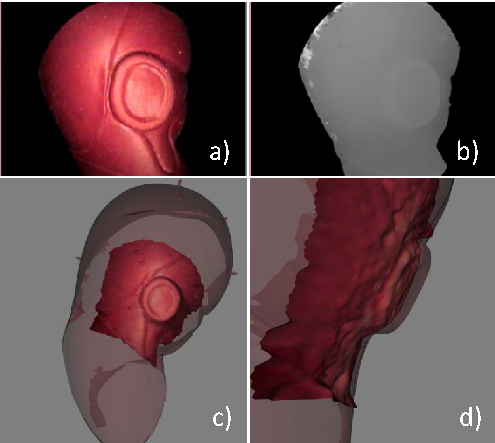
\includegraphics[width=0.5\textwidth]{SurfaceReconstructionStereoBased}
 \caption{Reconstruction of liver phantom. a) The phantom. b) Depth image. c)
   Initial overlap of the reconstructed point cloud with the tracked liver
   model. d) Side view \cite{speidel2011intraoperative}.}
  \label{fig:SurfaceReconstructionStereoBased}
\end{figure}

\subsection{Liver surface and vessels - Based on ultrasound}
This approach uses intraoperative ultrasound as the registration tool. It has
the advantage that inner and outer structures can be combined. Nam et al. \cite{nam2011automatic} take
advantage of the fact that the diaphragm can be made visible on ultrasound
images of the liver. At the same time also the vessels
are visible on the ultrasound images. Then they automatically segment the large
vessels and the part of the liver surface that is attached to the diaphragm.
They use the segmentation results to reconstruct the surface and some of the
vessels (Figure \ref{fig:VesselAndSurfaceRefinement}). Afterwards they merge the
reconstructed vessels and the surface to register to a preoperative model
(Figure \ref{fig:SurfaceAndVessel}).

% Automatic registration between 3D intra-operative ultrasound and pre-operative
% CT images \cite{nam2011automatic}

\begin{figure}[H]
  \centering
 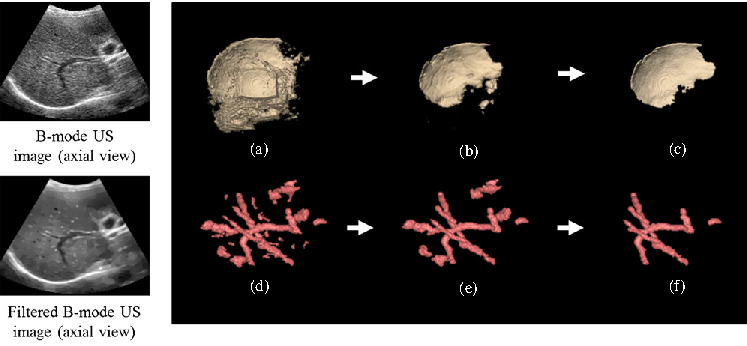
\includegraphics[width=0.8\textwidth]{VesselAndSurfaceRefinement}
 \caption{Automatic segmentation of the vessels and the surface from filtered 3D
   ultrasound images and the resulting step by step improved reconstruction \cite{nam2011automatic}.}
  \label{fig:VesselAndSurfaceRefinement}
\end{figure}

\begin{figure}[H]
  \centering
 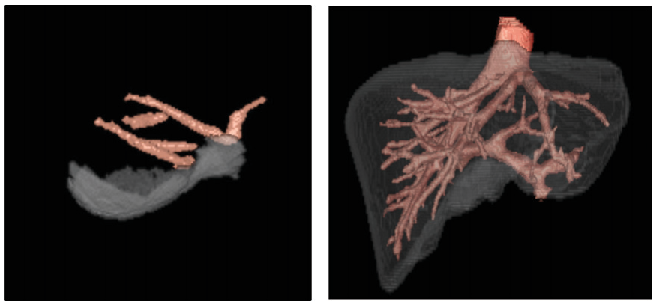
\includegraphics[width=0.8\textwidth]{SurfaceAndVessel}
 \caption{Left: The merged reconstruction of the vessels and the surface. Right:
   The whole liver reconstructed from a CT scan \cite{nam2011automatic}.}
  \label{fig:SurfaceAndVessel}
\end{figure}

% \subsection{Liver vessels - Based on ultrasound}
% Compounding of the US images to create a 3D US vessel model \cite{ribes2012image}



\section{Deficits of existing solutions}
From the last sections about the state of the art in navigation of liver
surgeries a few deficiencies  can be spotted. Regarding the ultrasound based
registrations, either the reviewed approaches
need a time consuming initial semi automatic alignment or have problems with the
compensation for deformations of the liver. 

Regarding the intraoperative creation of 3D models, some of these approaches lead to
incomplete models of the liver anatomy (only the surface). One approach creates
a 3D model of the liver surface and vessels using the intraoperative ultrasound.
But they use the created 3D model to register to a preoperative CT scan instead
of directly navigating using the intraoperatively created 3D model.

To conclude, registration based navigation approaches are error prone and
increase intraoperative complexity. So far, no system for liver surgeries allowing intraoperative creation of a 3D model and
its use for navigation afterwards exists. Such a system could decrease surgical
complexity by eliminating registration from the workflow.
% Assessment of Intraoperative Liver Deformation During Hepatic Resection:
% Prospective Clinical Study \cite{heizmann2010assessment}

% Projective biomechanical depth matching for soft tissue registration in
% laparoscopic surgery \cite{reichard2017projective}

\section{Objectives} 
To tackle the challanges described in the previous section, the
objectives of this Master's thesis are defined as follows:
\begin{itemize}
  \item Implementation of a concept for an intraoperative 3D reconstruction
  technique of the liver from intraoperative ultrasound. 
  \item Implementation of an intraoperative resection planning.
\end{itemize}
This work focuses on open surgical procedures of parenchymal-sparing liver resections.





% \begin{itemize}
%   \item not tracked laproscopic one shot images stereo with registration
%   \item moved laproscopic tracked endoscope stereo with registration 
% \end{list}

% \cite{hoppe1992surface}

% \section{Intraoperative ultrasound}
% \textcolor{green}{Start with why US is used, then describe how it works and the limitations. from there you should have a nice transition to navigation}
% In
% liver surgeries an intraoperative ultrasound device is used for intraoperative planning and
% navigation inside the liver. It is used to locate tumors that are not
% visible on the liver surface and to estimate their sizes from the ultrasound image. Figure \ref{fig:liverUS} shows an example of an
% ultrasound image of the liver and its corresponding position in the 3D liver
% model.

% \begin{figure}[H]
%   \centering
%  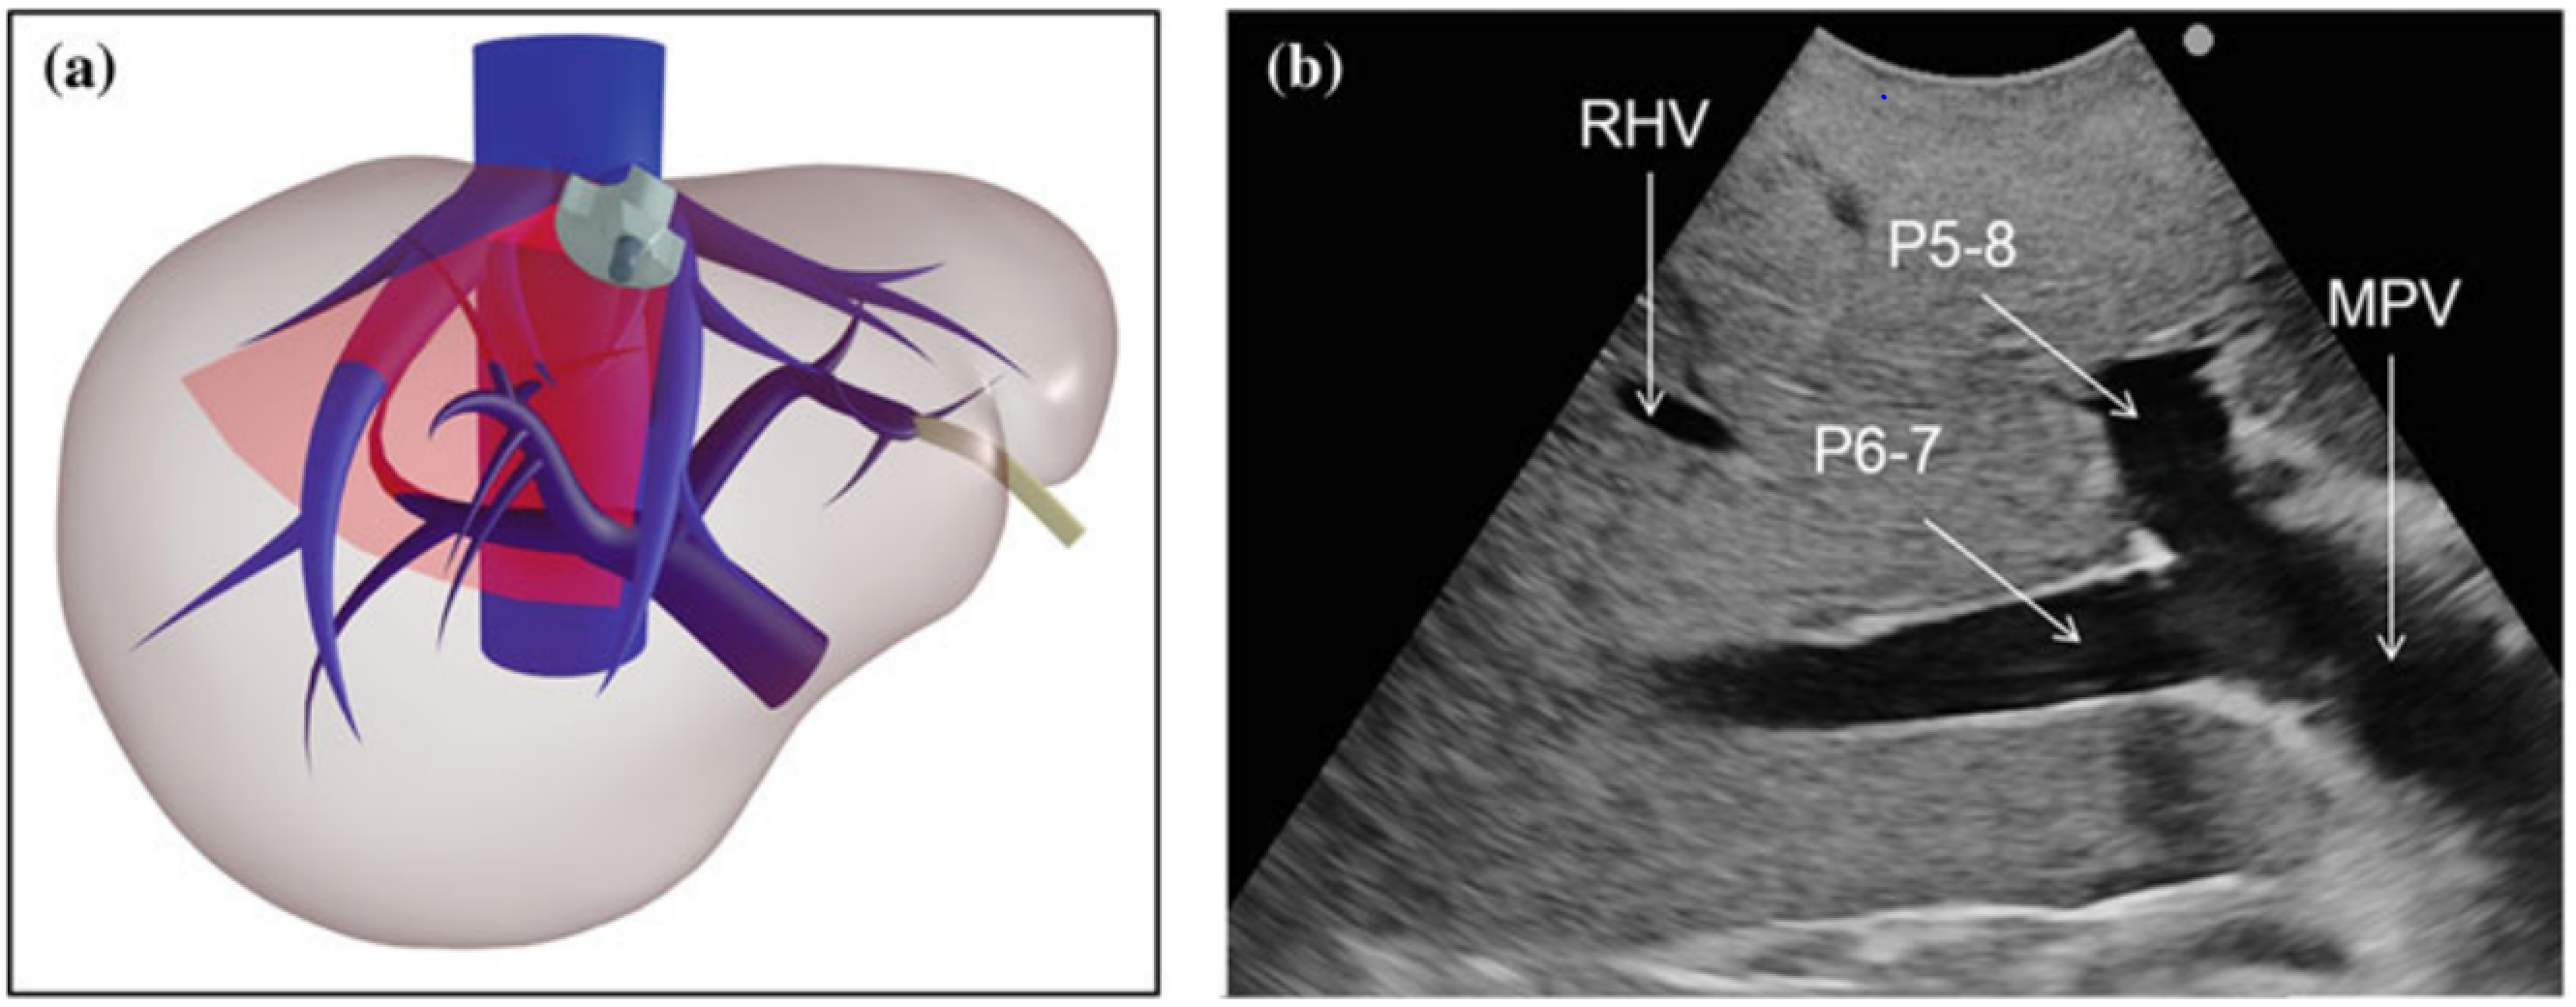
\includegraphics[width=\textwidth]{liverUS}
%  \caption{ Left (a) ultrasound image plane in the liver. Right (b) intraoperative
%    ultrasound image. One can see the right hepatic vein (RHV), the portal branch
%    to segments 5 and 8 (P5-8) and the portal branch to segments 6 and 7 (P6-7) \cite{torzilli2014ultrasound}}
%   \label{fig:liverUS}
% \end{figure}

% Ultrasound imaging works by the \textit{pulse-echo} principle. A short
% ultrasound pulse is emitted from a transducer. The sound waves get
% transmitted and reflected differently by different tissues. The reflected
%  waves travel back into the transducer and are converted into an electrical
% signal. After post-processing these signals become ultrasound images. 
% The ultrasound measures the mechanical properties of the tissue. The tissues
% have different acoustic impedance, which is the product of tissue density and
% ultrasound speed in travelling through the tissue. The resolution of the
% ultrasound images depends on the frequency of the ultrasonic waves. High
% frequencies lead to higher resolution but lower penetration depth into the tissue because the
% absorption of the sound energy increases with frequency too. Therefore the
% useability to see deep structures is limited \cite{torzilli2014ultrasound}. 

% In liver surgeries ultrasound is an important and established instrument.
% Intraoperatively, the ultrasound is used on the liver surface directly,
% therefore the penetration depth of the
% ultrasound is optimal to represent the inner structures of the liver.
% Registration methods based on 3D ultrasound reconstructed liver vessels 
% exist but are not used in practice frequently \cite{lange2003vessel}. Ultrasound
% is not harmful to health and therefore, can
% be used as often as desired to navigate during a surgery.
% % it is  
% % Intraoperatively surgeons use ultrasound to localize the tumor as it gives
% % advantages of reduced surgical time, complexity and radiation dosage.

% \section{Navigation for liver resections}
% \label{sec:navigationForLiverResections}
% \textcolor{green}{first, why is navigation needed, then how does it generally work
%   1) preoperative model or surgical plan 2) tracking 3) registration 4)
%   navigation visualization etc. then challenges especially in liver surgery and limitations}
% It is a difficult task for inexperienced surgeons to orientate themselves within the liver during an operation.
% From the outside of the liver it is not visible where the blood vessels are which they do not want to hurt.
% Navigation can help surgeons to orient themselves precisely in organs during
% operations.

% % The actual intervention in computer assisted surgeries (CAS) is defined as
% % surgical navigation.
% A navigated operation differs in a few points from a non-navigated operation.
% Because every patient's liver is different, a new 3D model of the liver has to
% be created before surgery. This models are created from pre-operative 3D
% computer tomography (CT) scan of the liver. Then, using this model, a surgical plan is made.
% In contrast to a regular operation, a navigation system is located in the
% operating theatre and the surgical instruments can be tracked by it. Therefore special instruments are used. These
% instruments have the ability to be tracked by the naviagation system. Depending
% on the tracking technology used by the navigation system, the tools are different.
% In order to also track the liver, the created model is registered to the anatomy
% of the patient. Finally the orientation and position
% of the instruments in relation to the patient's anatomy is visualized on a
% monitor in the operating room. The surgeon can see what he does on the
% monitor and uses the system to navigate the location and position of its
% instruments. This is specialy then useful when the tip of the instrument is not
% actually visible for the suergeon.

% The achieved
% navigation accuracy with such a system was 4.5 mm $\pm$3.6 mm averaged over nine surgeries \cite{peterhans2011navigation}.
% Current research tries to compensate for deformations of the liver after the CT
% scan to the actual shape of the liver \cite{clements2017deformation}
% \cite{clements2015validation}. 
% \subsection{Creation of preoperative 3D-models}
% Several steps are necessary to create a preoperative model. First the 
% CT scan is done. This leads to representations of the liver on several 2D images parallel
% to each other, filling a square volume with voxels. From this data the liver and
% its inner structures are manually segmented and merged to a 3D model (Figure \ref{fig:MeVisExample}). This is very
% time consuming and therefore expensive \cite{numminen2005preoperative}.
% Nevertheless the resulting models are very detailed and accurate.
% \begin{figure}[H]
%   \centering
%  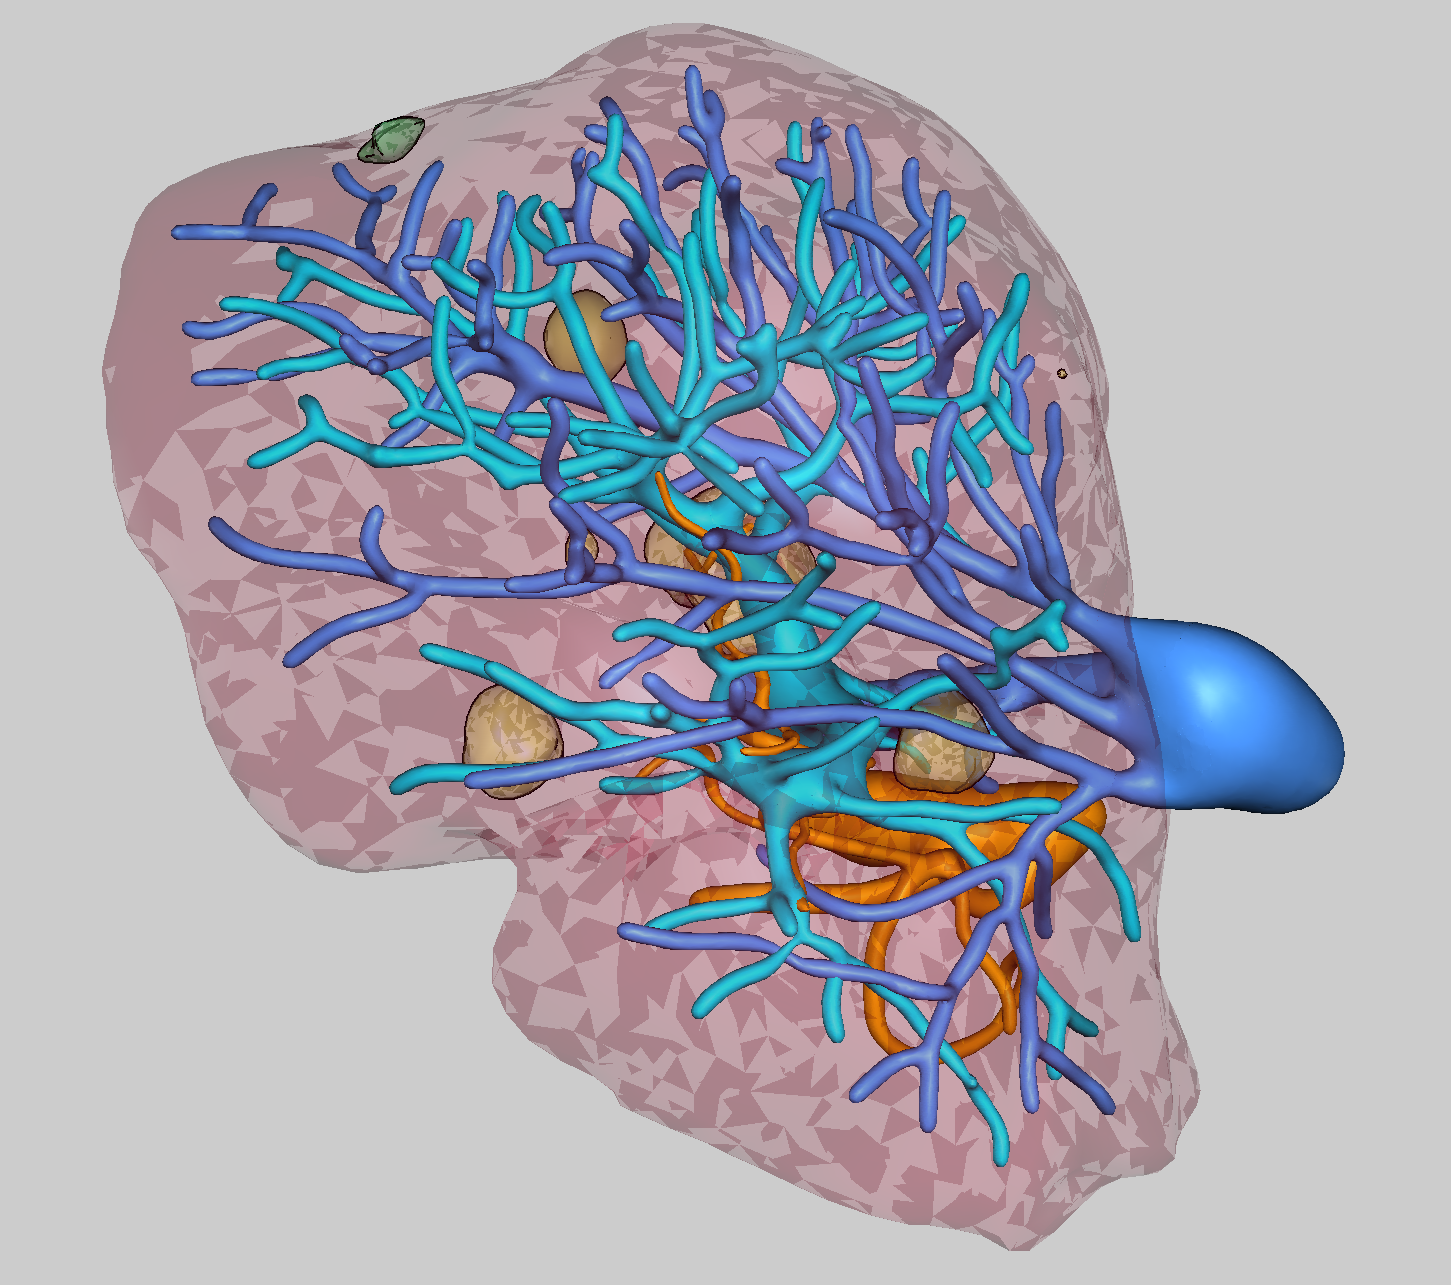
\includegraphics[width=0.6\textwidth]{MeVisExample}
%  \caption{Example of a preoperative 3D model created by MeVis}%DK patient
%   \label{fig:MeVisExample}
% \end{figure}

% \subsection{Registration methods}
% Patient registration is a concept to correlate the reference coordinate system
% of a virtual 3D data set with that of a patient. First, the 3D data set has to
% be gathered. This is often done by CT or MRI scan of the patients anatomy to be
% operated on. Secondly, finding of the transformation between the patient's
% reference coordinate system and the virtual data set. During the surgery the patient is similarly
% tracked as the instruments (see section \ref{sec:navigationForLiverResections}).
% In this way, the patient has his own coordinate system. From here many different
% methods exist to align the virtal data to the real anatomy.
% Discrete landmarks, surface scans and
% volumetric sonography scans are just a few of the approaches that can be
% used to achieve precise alignment of the data with the
% surgical site \cite{banz2016intraoperative}. 

% \subsubsection{Surface registration}
% Surface registration is registration based on surfaces. It is used and studied
% for several years in all kinds of fields \cite{ramos2015review}. Especially in
% the field of medical technology, a lot of research is being done in the
% direction of contactless registration. Intraoperatively, different camera technologies which lead
% to depth images are used to sample the surface of an organ. Often used imaging systems are stereo cameras
% \cite{furukawa2010accurate}, structured light \cite{salvi2004pattern} and
% laser range scanners \cite{cash2003incorporation}. From these intraoperatively
% created data sets, surfaces are reconstructed and then used for registration. To
% find the mapping between the surfaces, mostly different variants of the iterative
% closest point (ICP) \cite{besl1992method} algorithm are used. 

% These surface based methods are limited for different reasons. In most cases
% only part of the whole organ can be seen (scanned). The scanned surface may lack
% of unique structures on the surface. The scanning process can 
% lead to noisy data. The organ of interest may be deformed between the
% acquisitions of the surface samples. Therefore researchers try to compensate for
% intraoperative soft-tissue deformations \cite{cash2005compensating}\cite{dagon2008real}.
% \subsection{Tracking modalities}
% To track surgical instruments and patient's anatomy (define the position and
% orientation in real time) during naviagated surgery a tracking system is needed.
% Tracking can be done by different technologies. The most used tracking
% modality is optical tracking. 

% \subsubsection{Optical tracking}
% Optical tracking is the most used tracking modality in naviagated liver
% surgeries. Passive markers (spherical, retro-reflective that reflect infrared
% light) or active markers (infrared-emitting markers that are activated by an
% electrical signal) \cite{wiles2004accuracy} are attached to the objects that
% need to be tracked. A tracking camera is then emitting infrared light by illuminators
% on the position sensor (only for passive markers). The position sensor
% determines the position and orientation of the tracked instruments based on the
% information it receives from those markers \cite{noauthor_polaris_nodate}.  
\endinput
%%% Local Variables:
%%% TeX-master: "MscThesis"
%%% End: